\documentclass[a4paper]{article}

\usepackage{pgfplots}
\usepgfplotslibrary{smithchart}

\pgfplotsset{compat=1.5}

\begin{document}

%\tracingcommands=2\tracingmacros=2

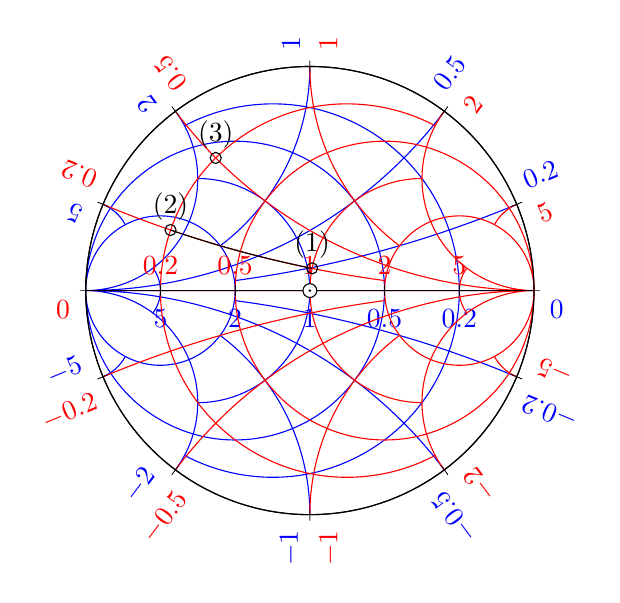
\begin{tikzpicture}[]
\begin{smithchart}[
	smithchart mirrored,
	xticklabel shift=-19pt,
	grid style={blue},
	ticklabel style={blue},
	yticklabel around circle,
]
\end{smithchart}

\begin{smithchart}[
	show origin,
	grid style={red},
	ticklabel style={red},
	yticklabel around circle*,
]
\addplot+[black,mark=o,only marks,point meta=explicit symbolic,nodes near coords]
coordinates {
	(0.2,0.2) [(2)]
	(1,0.2) [(1)]
	};

\addplot+[black,no marks,domain=0.2:1] {0.2};

\addplot+[black,mark=o,only marks,point meta=explicit symbolic,nodes near coords]
coordinates{
	(0.2,0.5) [(3)]
};
\end{smithchart}
\end{tikzpicture}
\end{document}

